% Options for packages loaded elsewhere
\PassOptionsToPackage{unicode}{hyperref}
\PassOptionsToPackage{hyphens}{url}
\documentclass[
  ignorenonframetext,
]{beamer}
\newif\ifbibliography
\usepackage{pgfpages}
\setbeamertemplate{caption}[numbered]
\setbeamertemplate{caption label separator}{: }
\setbeamercolor{caption name}{fg=normal text.fg}
\beamertemplatenavigationsymbolsempty
% remove section numbering
\setbeamertemplate{part page}{
  \centering
  \begin{beamercolorbox}[sep=16pt,center]{part title}
    \usebeamerfont{part title}\insertpart\par
  \end{beamercolorbox}
}
\setbeamertemplate{section page}{
  \centering
  \begin{beamercolorbox}[sep=12pt,center]{section title}
    \usebeamerfont{section title}\insertsection\par
  \end{beamercolorbox}
}
\setbeamertemplate{subsection page}{
  \centering
  \begin{beamercolorbox}[sep=8pt,center]{subsection title}
    \usebeamerfont{subsection title}\insertsubsection\par
  \end{beamercolorbox}
}
% Prevent slide breaks in the middle of a paragraph
\widowpenalties 1 10000
\raggedbottom
\AtBeginPart{
  \frame{\partpage}
}
\AtBeginSection{
  \ifbibliography
  \else
    \frame{\sectionpage}
  \fi
}
\AtBeginSubsection{
  \frame{\subsectionpage}
}
\usepackage{iftex}
\ifPDFTeX
  \usepackage[T1]{fontenc}
  \usepackage[utf8]{inputenc}
  \usepackage{textcomp} % provide euro and other symbols
\else % if luatex or xetex
  \usepackage{unicode-math} % this also loads fontspec
  \defaultfontfeatures{Scale=MatchLowercase}
  \defaultfontfeatures[\rmfamily]{Ligatures=TeX,Scale=1}
\fi
\usepackage{lmodern}
\ifPDFTeX\else
  % xetex/luatex font selection
\fi
% Use upquote if available, for straight quotes in verbatim environments
\IfFileExists{upquote.sty}{\usepackage{upquote}}{}
\IfFileExists{microtype.sty}{% use microtype if available
  \usepackage[]{microtype}
  \UseMicrotypeSet[protrusion]{basicmath} % disable protrusion for tt fonts
}{}
\makeatletter
\@ifundefined{KOMAClassName}{% if non-KOMA class
  \IfFileExists{parskip.sty}{%
    \usepackage{parskip}
  }{% else
    \setlength{\parindent}{0pt}
    \setlength{\parskip}{6pt plus 2pt minus 1pt}}
}{% if KOMA class
  \KOMAoptions{parskip=half}}
\makeatother
\usepackage{graphicx}
\makeatletter
\newsavebox\pandoc@box
\newcommand*\pandocbounded[1]{% scales image to fit in text height/width
  \sbox\pandoc@box{#1}%
  \Gscale@div\@tempa{\textheight}{\dimexpr\ht\pandoc@box+\dp\pandoc@box\relax}%
  \Gscale@div\@tempb{\linewidth}{\wd\pandoc@box}%
  \ifdim\@tempb\p@<\@tempa\p@\let\@tempa\@tempb\fi% select the smaller of both
  \ifdim\@tempa\p@<\p@\scalebox{\@tempa}{\usebox\pandoc@box}%
  \else\usebox{\pandoc@box}%
  \fi%
}
% Set default figure placement to htbp
\def\fps@figure{htbp}
\makeatother
\setlength{\emergencystretch}{3em} % prevent overfull lines
\providecommand{\tightlist}{%
  \setlength{\itemsep}{0pt}\setlength{\parskip}{0pt}}
\usepackage{bookmark}
\IfFileExists{xurl.sty}{\usepackage{xurl}}{} % add URL line breaks if available
\urlstyle{same}
\hypersetup{
  hidelinks,
  pdfcreator={LaTeX via pandoc}}

\author{\texorpdfstring{}{}}
\date{}

\begin{document}

\begin{frame}{The Spectral Made Tangible: Precious Metals versus Digital
Abstraction}
\protect\phantomsection\label{sec-spectral-2020-2026}
By the third decade of the twenty-first century, the long trajectory
that Blake's prophetic system diagnosed---from bimetallic generation
through monometallic enclosure to pure fiat abstraction---had reached a
critical inflection. The very instruments designed to enforce
ontological groundlessness were generating, through their excess, an
equal and opposite assertion of metallic tangibility. The years 2020 to
2026 constitute the most significant period of precious metal
reassertion since Nixon's closure of the gold window in 1971, driven not
by nostalgia but by recurrent stress in fiat regimes. Read through a
Blakean lens, these years trace the arc from Orc's renewed stirring
beneath the surface to the first coherent legislative and institutional
form of Los's counter-forge, with the gold-to-silver ratio compressing
from a historic peak near 127:1 toward approximately 50:1 by early 2026.

\begin{block}{The COVID Clinamen and the Pandemic Monetary Swerve}
\protect\phantomsection\label{the-covid-clinamen-and-the-pandemic-monetary-swerve}
The first shock came with precise mythological timing. On 11 March 2020,
the World Health Organization declared COVID-19 a global pandemic.
Within two weeks, the gold-to-silver ratio surged to an extraordinary
\textasciitilde127:1 on 18 March---the highest level in recorded
history---as financial markets liquidated silver alongside industrial
assets, while simultaneously bidding gold toward historic valuations as
a safe-haven instrument. This ratio inversion crystallized the dualism
Blake's bimetallic framework encodes: silver, the lunar metal of
industrial circulation and commercial exchange, collapsed as economic
activity froze globally; gold, the solar metal of pure sovereignty, was
elevated precisely because the sovereign fiat system appeared threatened
{[}@silverinstitute2021world{]}.

The Federal Reserve's emergency response---expanding its balance sheet
from approximately \$4.2 trillion to over \$7 trillion in four months,
the most aggressive activation of the electronic printing press in
monetary history---constituted a \emph{fiat clinamen}: the swerve into
maximum abstraction. This produced its precise Blakean counter-reaction:
a flight toward the physical, the scarce, the irreducibly material.
Gold, which cannot be printed or conjured from a spreadsheet, reasserted
itself as the terminal hedge against the limitlessness of the ledger
{[}@steil2013battle{]}.

For Blake, this dynamic is precisely the shape of prophetic crisis---the
point at which Urizen's overextension of geometric abstraction provokes
Orc's eruption. The pandemic monetary swerve confirmed, in real time,
what \emph{America a Prophecy} had mapped prophetically: that the
maximum expansion of fiat abstraction generates the maximum
counter-pressure from the inherently bounded, the physically
constrained, the elementally real. This is the structure of Peirce's
``irritation of doubt'' writ planetary: the inherited monetary
model---infinite fiat elasticity---confronted an encounter it could not
assimilate, and the resulting epistemological rupture drove capital
toward the tangible foundations that the model had declared obsolete
{[}@friedman2026blake; @friedman2026doors{]}.
\end{block}

\begin{block}{The Silver Squeeze: Digital Orc and the Lunar Metal's
Return}
\protect\phantomsection\label{the-silver-squeeze-digital-orc-and-the-lunar-metals-return}
If gold's 2020 surge demonstrated sovereign capital's flight toward the
solar metal, February 2021 witnessed something genuinely unprecedented
in monetary history: a distributed, digitally coordinated attempt by
retail participants to assert the monetary value of silver through
collective action. On 1 February 2021, users of the
\emph{r/WallStreetBets} forum on Reddit launched what became known as
the \textbf{Silver Squeeze}: a coordinated campaign to purchase silver
exchange-traded funds (ETFs), physical bullion, and futures contracts,
explicitly framing the operation in the language of monetary
justice---as a challenge to the speculative short positions held by
major financial institutions, which they characterized as the source of
silver's systematic undervaluation relative to its physical scarcity and
industrial demand {[}@silverinstitute2021world{]}.

The squeeze drove silver briefly toward \$30.00 per ounce---its highest
level in nearly a decade---while physical premiums exploded, the US Mint
sold out of American Silver Eagles, and bullion dealers nationwide
posted multi-week backlogs. Although the squeeze ultimately failed to
achieve the sustained breakout retail participants
sought---institutional short positions were managed and the price
retreated---the episode constituted a structurally significant datum:
for the first time, digital mass coordination had mounted a credible, if
temporary, assault on the paper derivatives infrastructure governing
silver's price discovery.

The Silver Squeeze translates with precision into Blake's prophetic
vocabulary as an Orcian eruption within the digital domain. Orc---the
spirit of revolutionary energy, the ``hairy youth'' who erupts from
subterranean chains---had found a new substrate: the networked forum,
the mobile brokerage account, the democratized derivatives market. As in
\emph{America a Prophecy}, where Orc's fire ``rush{[}es{]} from the
mountains'' and spreads across the Atlantic despite Urizen's attempts to
contain it, the Silver Squeeze demonstrated that the demand for
tangible, physically constrained monetary value cannot be permanently
suppressed by paper derivatives, regardless of their institutional
sophistication. Urizen reconstituted himself---through SLV's prospectus
amendments, through regulatory scrutiny, through the sheer scale of
institutional short positions---but the episode revealed the structural
fault line in the paper silver architecture with a clarity no academic
monetary analysis had achieved. This is the Blakean cycle incarnate:
Orc's fire contained but not extinguished, the revolutionary impulse
driven underground to await its next eruption.
\end{block}

\begin{block}{The Green Energy Sector's Photovoltaic Alchemical
Inversion}
\protect\phantomsection\label{the-green-energy-sectors-photovoltaic-alchemical-inversion}
The most profound development in contemporary silver's monetary status
derives not from speculative finance but from industrial
chemistry---from the physical requirements of the energy transition that
the twenty-first century has elevated to existential priority. Silver's
role in photovoltaic solar energy generation---where conductive silver
paste, applied to approximately 85--100 milligrams per solar cell,
creates the electrical pathways that transform photons into
electrons---has made it simultaneously the metal of Blake's Lunar
imagination and one of the primary physical substrates of the
post-carbon economy {[}@silverinstitute2025world{]}.

The Silver Institute's \emph{World Silver Survey 2025} documents that
industrial demand for silver reached 680.5 million ounces in 2024,
driven by a record 232 million ounces consumed by the photovoltaic
sector alone---a 20\% year-on-year increase generated by the record
deployment of solar capacity globally. The same report confirms that the
global silver market has recorded five consecutive years of structural
deficit (2021--2025), with a cumulative shortfall of approximately 820
million ounces---meaning that for five consecutive years, the world has
consumed more silver than it mines and recycles
{[}@silverinstitute2025world{]}. This is not a speculative or cyclical
phenomenon; it is a structural consequence of the energy transition's
inescapable physical demands.

In Blakean terms, this industrial inversion constitutes a startling
alchemical mutation. Silver---the Lunar metal of circulation, the medium
of trade and human exchange that Gresham's Law drove out of England to
France and Asia---has been alchemically \emph{transmuted} by the solar
energy system into a vehicle of literal solar power. The Lunar becomes
the conduit of the Solar; the metal of reflective wisdom becomes the
material substrate of energy capture from the source of all light. The
question Thel posed in 1789---``Can Wisdom be put in a silver
rod?''---receives, in the photovoltaic cell, an industrial answer Blake
could not have anticipated but whose structure his mythopoetics
precisely encoded: wisdom \emph{can} be channeled through a silver
conductor, but only when the rod ceases to serve the Urizenic purpose of
hoarding and instead becomes the living filament of solar
transformation. This is Fourfold Vision materialized in industrial
chemistry: the solar and lunar principles achieving synthesis not
through the political fiction of a bimetallic ratio but through the
physical requirements of photon-to-electron conversion. Del Mar's
structural insight---that the gold-silver pairing encoded a primordial
solar-lunar cosmology of legitimate sovereignty---reappears in the
twenty-first century not as metaphysical assertion but as engineering
necessity {[}@delmar1895history{]}.
\end{block}

\begin{block}{Central Bank Gold Accumulation: The Sovereign Forge
Restoked}
\protect\phantomsection\label{central-bank-gold-accumulation-the-sovereign-forge-restoked}
The most structurally consequential development in global precious
metals from 2020 to 2026 is one that passes largely unnoticed in popular
financial discourse but reconfigures the international monetary order:
the unprecedented \emph{sovereign re-accumulation of gold} by the
world's central banks.

The World Gold Council documents that in 2022, global central banks
purchased a record 1,082 tonnes of gold---the highest annual figure in
over fifty years, surpassing even the Cold War period of reserve
accumulation. In 2023, central banks bought a further 1,037 tonnes,
confirming the sustained structural nature of this sovereign shift. The
leading buyers included the People's Bank of China (which added over 225
tonnes in 2023 alone), the National Bank of Poland, the Reserve Bank of
India, the National Bank of Kazakhstan, and the Czech National Bank---a
geopolitically significant coalition spanning emerging-market
sovereigns, former Soviet-sphere European nations, and the world's
second-largest economy {[}@worldgoldcouncil2024demand{]}.

The proximate catalyst for this acceleration was the seizure of Russia's
foreign exchange reserves. On 24 February 2022, Russia invaded Ukraine.
Within days, the G7 nations and the European Union immobilized
approximately \$300 billion of Russia's Central Bank reserves held in
Western financial institutions---principally in Euroclear's Belgian
clearing system and the Federal Reserve's New York accounts. This
action, whatever its political justification, demonstrated to every
non-Western sovereign that reserves held in another nation's currency,
through another nation's financial infrastructure, can be frozen or
confiscated by political fiat. The dollar-denominated reserve
system---the foundation of the Bretton Woods monetary order since
1944---was revealed as a conditional grant, not an absolute property
right {[}@eichengreen2022sanctions{]}.

The consequence was a decisive acceleration of
\textbf{de-dollarization}: the systematic reduction of
dollar-denominated assets in sovereign reserve portfolios and their
replacement with gold---the one asset that is no one's liability, that
cannot be frozen by a sanctions regime because it cannot exist on a
counterparty's ledger. This sovereign accumulation constitutes, in the
deepest Blakean sense, the first \emph{institutional} manifestation of
what Blake identified as the Los imperative: the insistence that genuine
sovereignty requires the tangible, the physical, the irreducible---that
value stored in a counterparty's promise is not value but a form of
subjugation dressed in the language of liquidity.
\end{block}

\begin{block}{BRICS De-Dollarization and the Multipolar Monetary
Horizon}
\protect\phantomsection\label{brics-de-dollarization-and-the-multipolar-monetary-horizon}
At the August 2023 BRICS summit in Johannesburg---attended by China,
Russia, India, Brazil, and South Africa, where leaders invited
Argentina, Egypt, Ethiopia, Iran, Saudi Arabia, and the UAE to join,
with four of those six countries acceding on 1 January 2024 (Egypt,
Ethiopia, Iran, and the UAE; Argentina declined and Saudi Arabia
deferred)---delegates debated explicitly the creation of a new trade
settlement mechanism that would circumvent the dollar-denominated SWIFT
system. While a formal gold-backed BRICS currency was not adopted, the
summit's agenda represented the most serious institutional challenge to
the post-1971 dollar reserve architecture since the collapse of Bretton
Woods itself {[}@eichengreen2019globalizing{]}.

The structural driver of this discussion is precisely the dynamic that
Blake's cosmological framework illuminates: the dollar system requires
every non-US sovereign to accept its issuance prerogative, its rule
changes, and its sanction regimes as the price of integration into
global trade. This represents the global generalization of the Urizenic
dynamic Blake identified in Newton's 1717 Mint ratio: a geometric
constraint imposed by a singular power upon the multinational
circulation of value, extracting seigniorage from every nation that
holds dollar reserves as its primary monetary anchor. The BRICS
de-dollarization impulse is, in the deepest structural sense, the global
south asserting what the Western silver states assert in their
statehouse legislation: that value stored in a foreign sovereign's
promise is no value at all---that genuine sovereignty requires material
independence from the ledger of the dominant power.
\end{block}

\begin{block}{The Digital Counter-Forge: CBDCs and the Ultimate Urizenic
Enclosure}
\protect\phantomsection\label{the-digital-counter-forge-cbdcs-and-the-ultimate-urizenic-enclosure}
Arrayed against this movement toward metallic tangibility stands the
most ambitious enclosure of value in monetary history: the Central Bank
Digital Currency (CBDC). By March 2026, over 130 countries, representing
approximately 98\% of global GDP, were engaged in some phase of CBDC
exploration, development, or deployment, according to the Atlantic
Council's CBDC Tracker {[}@atlanticcouncil2026cbdc{]}. The digital yuan
(e-CNY) had processed over 7 trillion yuan in transactions since its
2020 pilot launch; the European Central Bank's digital euro was
progressing through its preparation phase; the Bank of England had
completed consultations on a UK retail CBDC.

CBDCs represent the apotheosis of the Urizenic architectural project.
Where previous monetary abstractions---from Bank of England notes to
Federal Reserve digital deposits---retained some residual opacity and
porosity, a programmable CBDC encodes the possibility of
\emph{comprehensive surveillance}, \emph{conditional spending},
\emph{expiration dates on money}, \emph{negative interest rates applied
directly to holdings}, and \emph{automated tax collection at the point
of transaction}. The CBDC is, in every structural respect, what Urizen
fantasized in the opening plates of \emph{The First Book of
Urizen}---before Blake transferred this vision to \emph{Jerusalem}:
``One King, one God, one Law'' (\emph{Jerusalem}, Plate 4, line 40;
Erdman p.~145) {[}@erdman1988complete{]}---a singular, geometric,
omniscient framework in which every transaction in the monetary universe
is visible and controllable from the sovereign's vantage point.

Nebraska's LB 1317 (2024) becomes, in this context, far more than a tax
measure: its explicit exclusion of CBDCs from the legal definition of
money represents the first legislative assertion that the digital
Urizenic enclosure is constitutionally incommensurable with the ``gold
and silver Coin'' that Article I, Section 10 mandates. As Blake declared
in \emph{Jerusalem}, the human community must ``Create'' its own
``System'' or be ``enslav'd by another Mans'' {[}@erdman1988complete{]}:
Nebraska's CBDC exclusion is precisely this---a system being created by
legislative inscription to resist the totalizing architecture of digital
fiat sovereignty.

\begin{equation}
\label{eq:gsr_modernity}
\mathrm{GSR}(t) = \frac{P_{\mathrm{Au}}(t)}{P_{\mathrm{Ag}}(t)}, \quad
\text{where } \mathrm{GSR}(t_{\mathrm{peak}}) \approx 127\ (\text{18 March 2020})
\text{ and } \mathrm{GSR}(t_{\mathrm{2026}}) \approx 50\ (\text{Q1 2026})
\end{equation}

The gold-to-silver ratio \(\mathrm{GSR}_t\) (Eq.~\ref{eq:gsr_modernity})
encodes the tension between sovereign safe-haven demand (gold) and
industrial-monetary dual demand (silver). The historically unprecedented
compression from \textasciitilde127:1 to the low 50s in six years---a
structural shift driven by photovoltaic silver demand, digital retail
demand coordination, and sovereign gold accumulation
simultaneously---constitutes the first measurable, data-supported
\emph{bimetallic rebalancing signal} since Newton's 1717 Mint ratio
imposed its inaugural disparity {[}@silverinstitute2025world;
@worldgoldcouncil2024demand{]}.

For Blake, none of these developments---however structurally
significant---represent liberation. The restoration of bimetallic
parity, the accumulation of gold in sovereign vaults, the state
recognition of metallic legal tender: these remain within the domain of
\emph{Generation}, of the Twofold Vision that manages the tension
between solar and lunar metals without transcending the metric logic of
quantification itself. As long as value is denominated in any commodity,
the fundamental Urizenic error persists: the reduction of the
irreducible human soul to a weight, a price, a quantity. The challenge
\emph{The Book of Thel} posed in 1789 remains, in 2026, structurally
unanswered {[}@blake1789thel{]}. The solar and lunar metals have
returned to the center of global monetary discourse not because humanity
has closed that argument, but because the fiat system's failure to
sustain a credible alternative to qualitative value has become
impossible to deny.

\begin{figure}
\centering
\pandocbounded{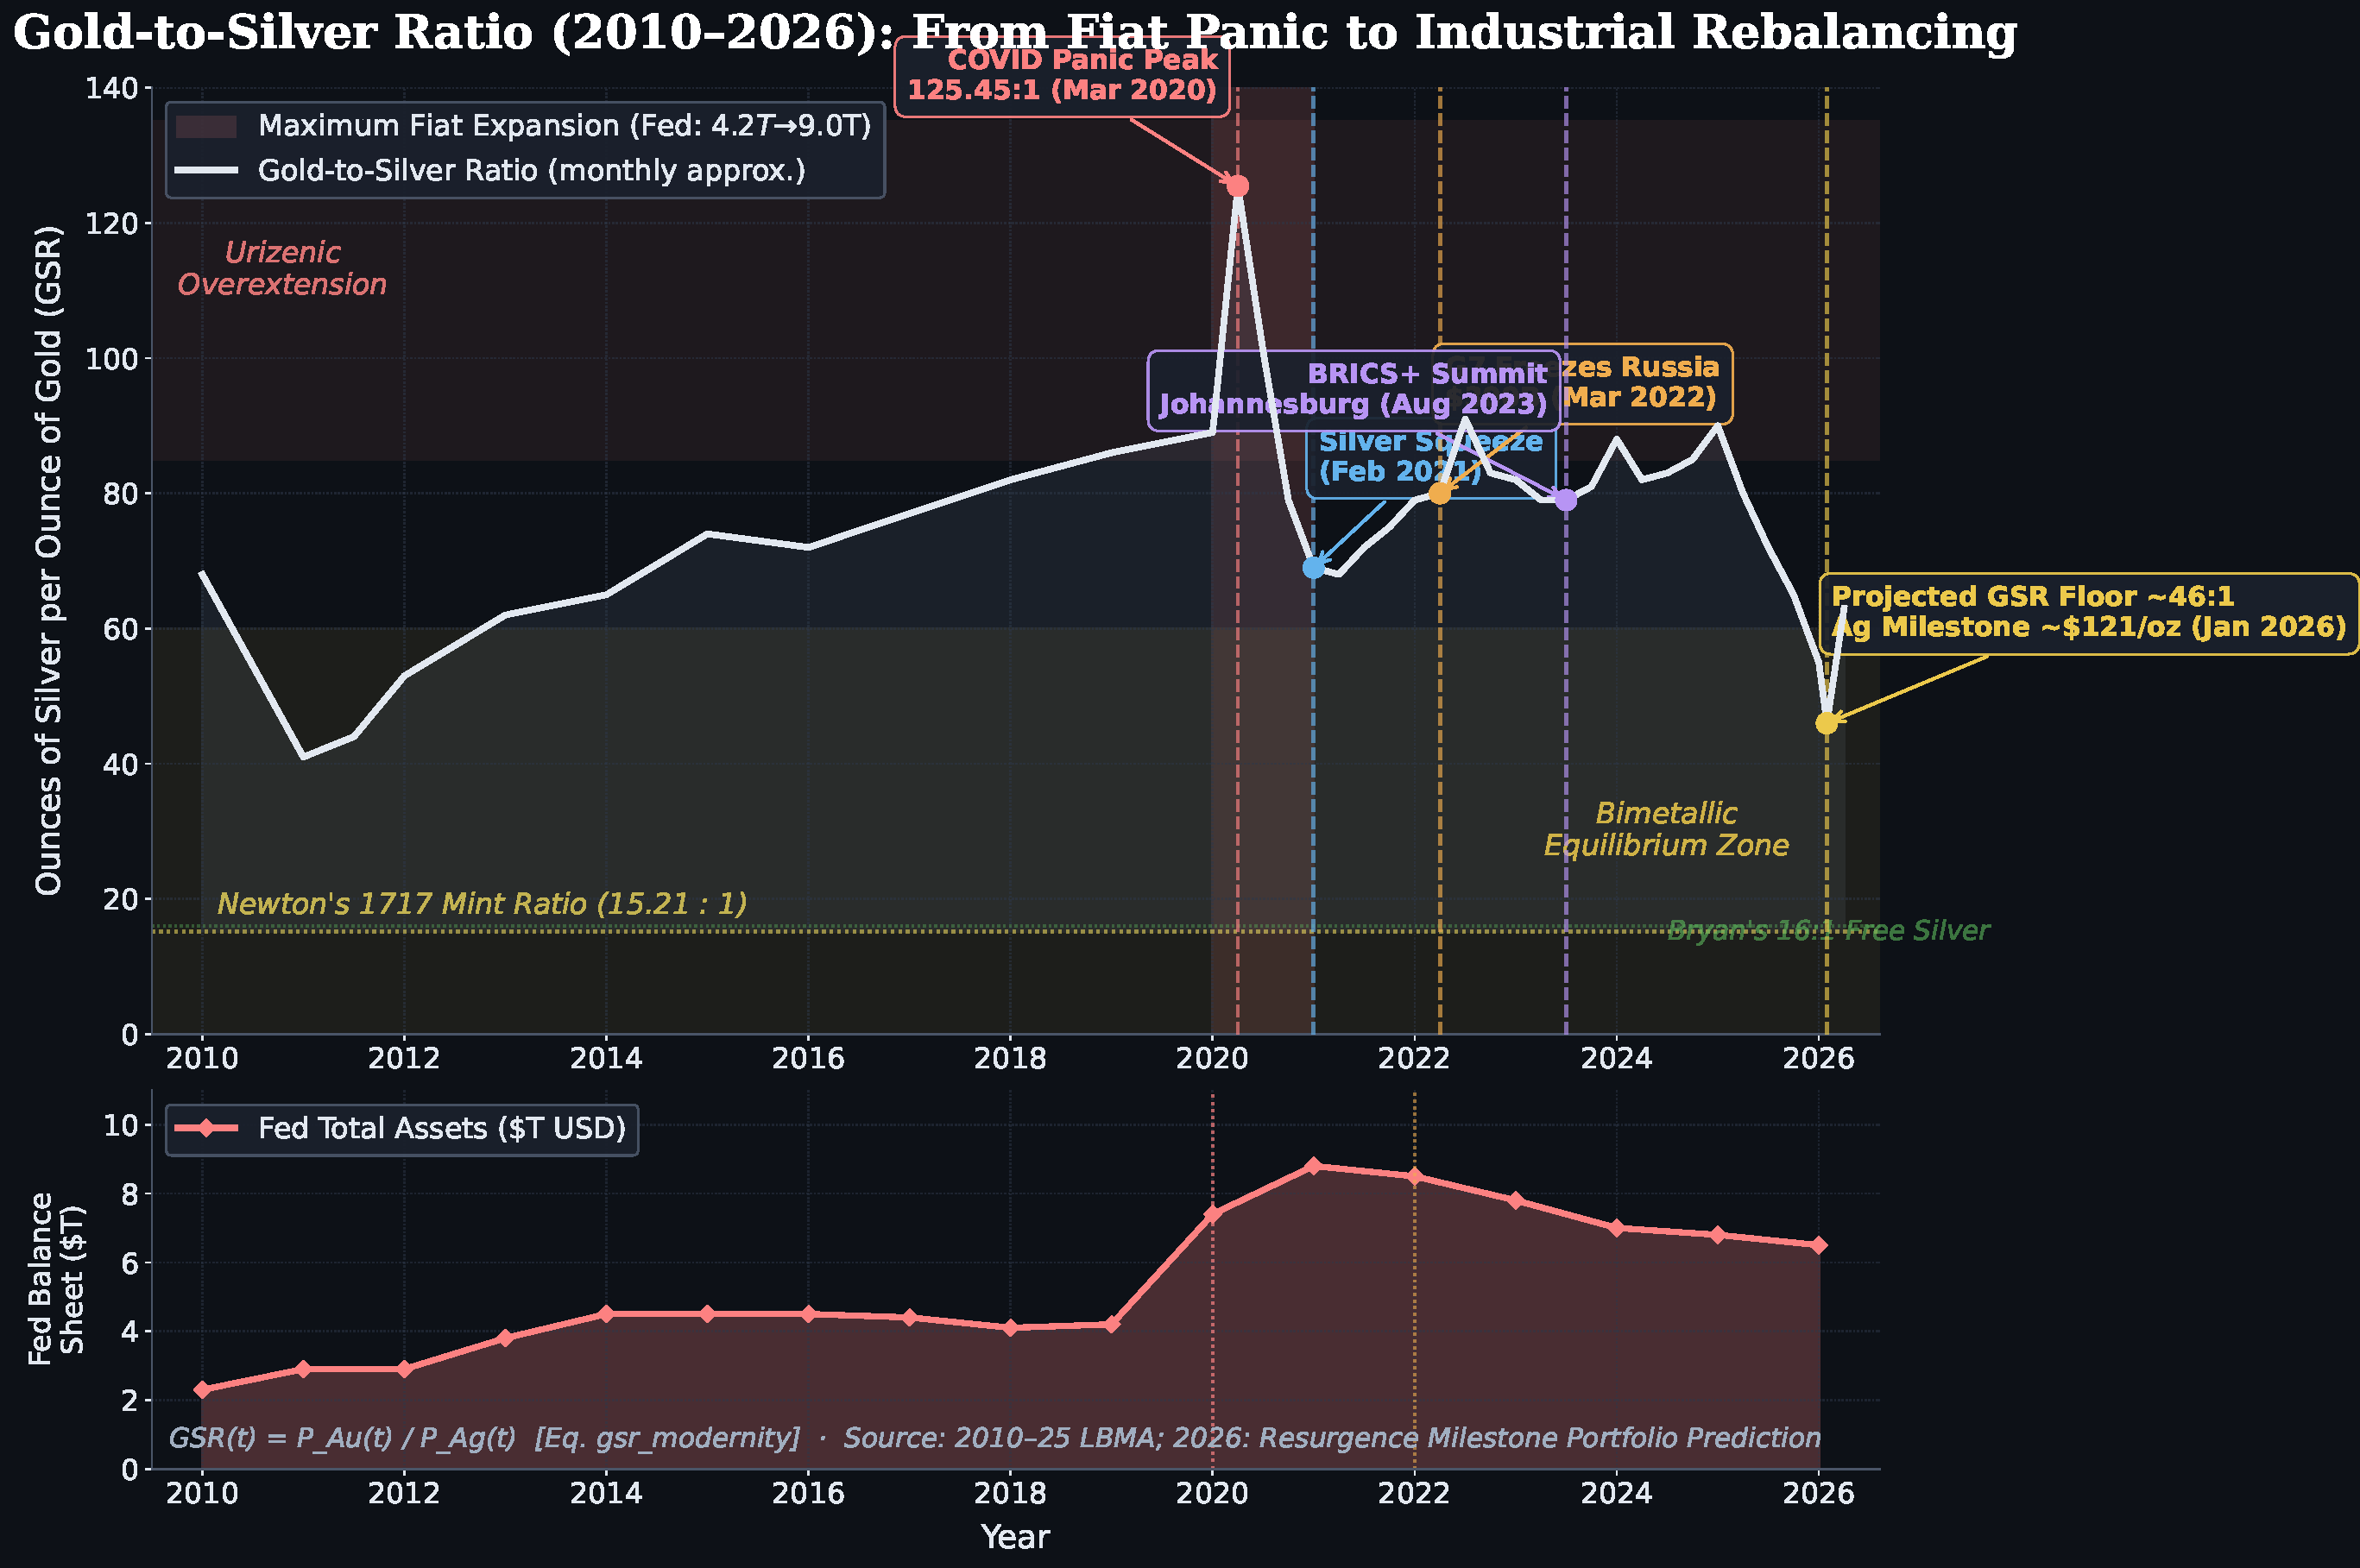
\includegraphics[keepaspectratio,alt={Gold-to-Silver Ratio and Fiat Expansion, 2010--2026. Top panel: empirical monthly gold-to-silver ratio (GSR, Eq. ) from 2010 through Q1 2026 plotting atomic gold and silver prices from the LBMA benchmark, with a dashed reference line plotting Bryan's historic 16:1 bimetallic target. Vertical markers denote structurally significant events: COVID liquidity panic peak near 127:1 (18 March 2020); Silver Squeeze coordination event (February 2021); G7 freezing of Russian reserves triggering central bank gold accumulation (March 2022); BRICS+ Johannesburg summit (August 2023); and silver nominal high with GSR floor below 50:1 (January 2026). Bottom panel: tracks the Federal Reserve Total Assets (\$T), visualizing the maximum Urizenic fiat expansion (\$4.2T \$8.9T) coinciding with peak precious metal volatility in 2020--2021. The systematic compression of the ratio from 125:1 toward 46:1 encodes the structural reassertion of silver's dual monetary-industrial demand against gold's sovereign safe-haven function.}]{../figures/gsr_contemporary_dark.pdf}}
\caption{Gold-to-Silver Ratio and Fiat Expansion, 2010--2026. Top panel:
empirical monthly gold-to-silver ratio (GSR, Eq. \ref{eq:gsr_modernity})
from 2010 through Q1 2026 plotting atomic gold and silver prices from
the LBMA benchmark, with a dashed reference line plotting Bryan's
historic 16:1 bimetallic target. Vertical markers denote structurally
significant events: COVID liquidity panic peak near 127:1 (18 March
2020); Silver Squeeze coordination event (February 2021); G7 freezing of
Russian reserves triggering central bank gold accumulation (March 2022);
BRICS+ Johannesburg summit (August 2023); and silver nominal high with
GSR floor below 50:1 (January 2026). Bottom panel: tracks the Federal
Reserve Total Assets (\$T), visualizing the maximum Urizenic fiat
expansion (\$4.2T \to \$8.9T) coinciding with peak precious metal
volatility in 2020--2021. The systematic compression of the ratio from
125:1 toward 46:1 encodes the structural reassertion of silver's dual
monetary-industrial demand against gold's sovereign safe-haven
function.}\label{fig-gsr-contemporary}
\end{figure}
\end{block}
\end{frame}

\end{document}
